\documentclass[11pt,a4paper]{moderncv}
\usepackage{pdfpages}
\usepackage{import} \import{./}{setup.tex}

\name{Federico}{del Mazo}
\title{
    \spa{Curriculum Vitae}
    \en{Résumé}
}
\address{Beruti 545, Ramos Mejía (1704)}
\phone[mobile]{+54 911 6110 1997}
\phone[fixed]{011 4656 4494}
\email{fdelmazo@fi.uba.ar}
\extrainfo{\faLinkedin \vspace{0.4mm} f • \faGithub \vspace{0.4mm} FdelMazo}
\quote{
    \spa{21 años, estudiante de ingeniería en informática.}
    \en{21 years old, computer engineering student.}
}

\begin{document}

\begin{picture}(0,0)
\put(-30,-110){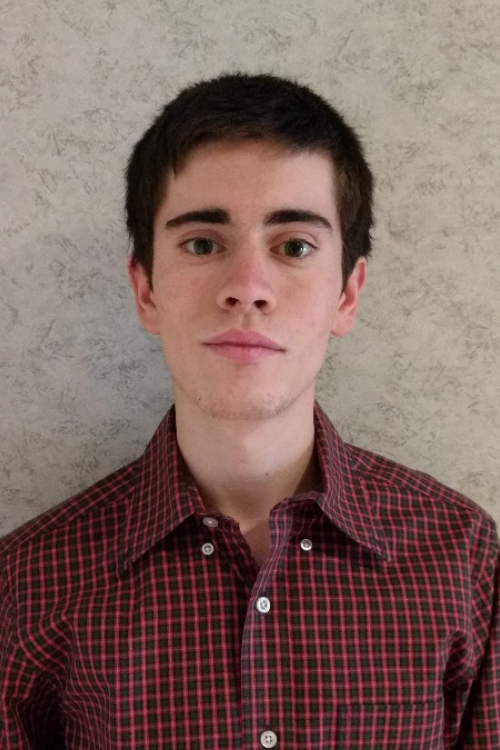
\includegraphics[scale=0.20]{fotoCV}}
\end{picture}

\thispagestyle{onlyfooter}

\makecvtitle
\addtolength{\parskip}{6pt}

\spa{Joven estudiante en busca de iniciarse en el mercado laboral con el objetivo de enriquecer sus conocimientos y desarrollarse en sus primeras experiencias profesionales.}
\en{Young student eager to delve deep into the IT industry and looking forward to improve his knowledge and skills.}

\section{\spa{Experiencia Laboral}\en{Work Experience}}

\cventry
    {\spa{Abril 2018--Actualidad}\en{April 2018--Now}}
    {\spa{Desarrollador de software}\en{Software developer}}
    {Raico S.A.}{}{}{https://www.raiconet.com/}

\section{\spa{Experiencia Laboral No Rentada}\en{Non-paid Work Experience}}

\cventry
    {\spa{Agosto 2017--Actualidad}\en{August 2017--Now}}
    {\spa{Ayudante de}\en{Adjunct professor in} Algoritmos y Programación II - Curso Wachenhauzer}
    {Universidad de Buenos Aires, Facultad de Ingeniería}{}{}{https://algoritmos-rw.github.io/algo2/}

\section{\spa{Educación}\en{Education}}

\cventry
    {\spa{2015--Actualidad}\en{2015--Now}}
    {\spa{Estudiante de Ingeniería en Informática}\en{Computer engineering student}}
    {Universidad de Buenos Aires, Facultad de Ingeniería}{}{}{}

\cventry
    {2009--2014}
    {\spa{Bachiller Bilingüe en Economía y Administración}\en{Bilingual bachelors' degree in economics and business administration}}
    {Colegio Ward}{}{}{\textit{\spa{Promedio general}\en{Grade Point Average} 8.29}}

\cventry
    {2012--2013}
    {International General Certificate of Secondary Education (IGCSE)}
    {University of Cambridge}{}{}{\textit{Passed with Merit}}
%     Environtmental Management B
%     Geography B
%     First Language Spanish D
%     Economics B
%     Mathematics B
%     Business Studies C
%     First language english D

\cventry
    {2011}
    {First Certificate in English}
    {University of Cambridge}{}{}{\textit{Grade C}}
% Cambridge ESOL Level 1 Certificate in ESOL International

\section{\spa{Conocimientos específicos}\en{Specific skills}}

\begin{itemize}
\item \textbf{\spa{Lenguajes de programación}\en{Programming languages}:} C, Python, Java, JavaScript, SmallTalk, Lua.
\item \textbf{\spa{Otros lenguajes}\en{Other languages}:} SQL, TeX, HTML, CSS, UML.
\item \textbf{\spa{Otros}\en{Other}:} jQuery, Bootstrap, Groovy, Grails.
\end{itemize}

\section{\spa{Intereses y actividades extracurriculares}\en{Interests and extracurricular activities}}

\begin{itemize}
\item
    \spa{\textbf{Programación} Todos mis proyectos personales (videojuegos, programas) pueden verse en mi perfil de Github.}
    \en{\textbf{Programming} All of my personal projects (videogames, programs) can be seen on my Github profile.}

\item 
    \spa{\textbf{Cine} Desde siempre tengo una pasión por el cine y asistí a diversos talleres y cursos:
        \begin{itemize}
            \item{Jornada IV de Antropología e Imagen - Facultad de Filosofia y Letras de la UBA}
            \item{Introducción al septimo arte, por Sebastián de Caro - Universidad CAECE}
            \item{Realización cinematográfica, por Mariano Swi - CC Matienzo}
        \end{itemize}
    }
    \en{\textbf{Cinema} I have always been interested in cinema and film and have attended several workshops and courses:
        \begin{itemize}
            \item{Jornada IV de Antropología e Imagen - Facultad de Filosofia y Letras de la UBA}
            \item{Introduccion al septimo arte, by Sebastián de Caro - Universidad CAECE}
            \item{Realización cinematográfica, by Mariano Swi - CC Matienzo}
        \end{itemize}
    }

\item
    \spa{\textbf{Deportes} Entre los 10 y 17 años me desempeñé en handball en el equipo del Colegio Ward, saliendo campeón y subcampeón en distintas competencias de la Federación Metropolitana de Balonmano.}
    \en{\textbf{Sports} Between the ages of 10 and 17 I've been a handball player in Colegio Ward winning several tournaments and leagues of the Federación Metropolitana de Balonmano.}

\item
    \spa{\textbf{Música} Entre los 12 y 18 años participé en la Banda del Colegio Ward tocando la trompeta y el piano. Con esta fuí a diversas convenciones musicales de Argentina.}
    \en{\textbf{Music} Between the ages of 12 and 18 I've been a trumpet and piano player in Colegio Ward attending several music conventions in Argentina.}

\end{itemize}

\IfFileExists{./notas.pdf}{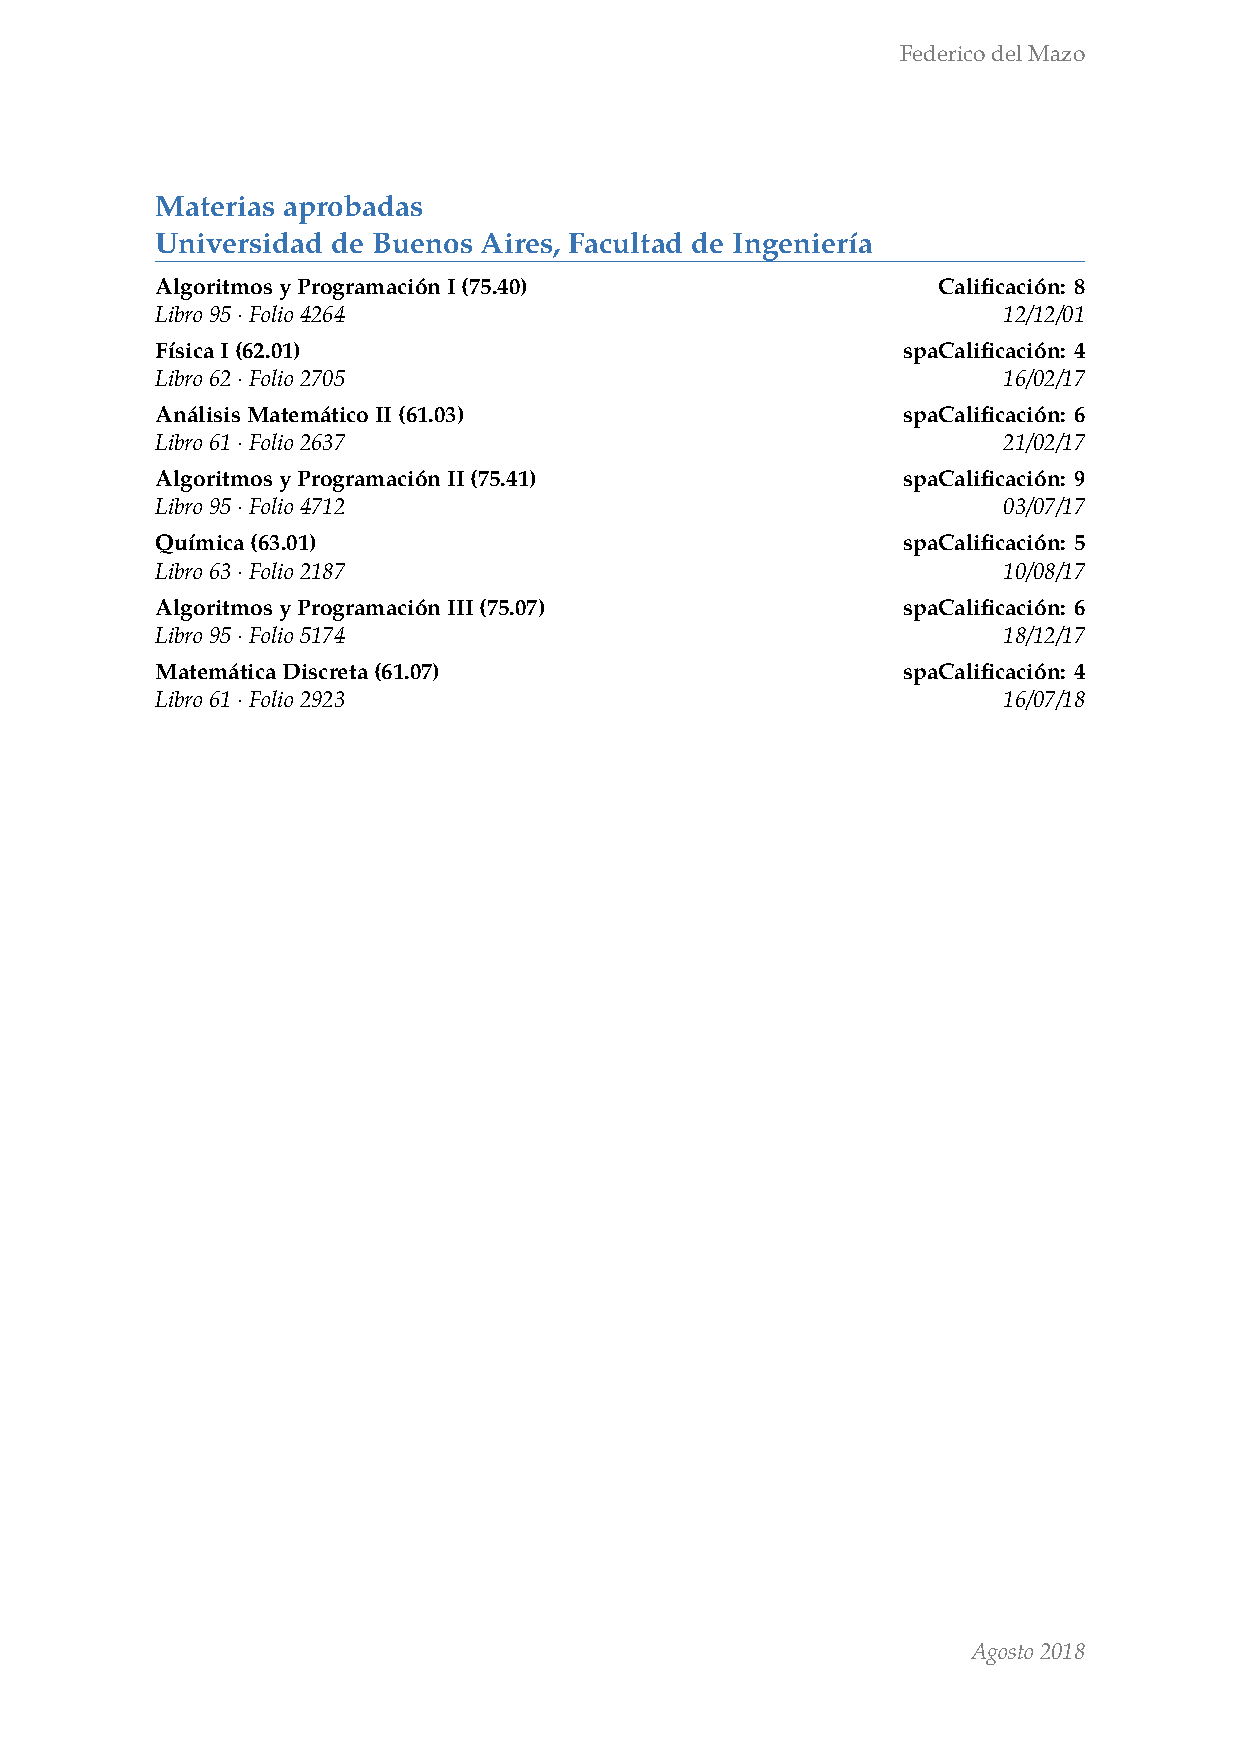
\includepdf[pages=-]{notas.pdf}}{}
\end{document}

